\documentclass[12pt]{article}
\setlength{\oddsidemargin}{0in}
\setlength{\evensidemargin}{0in}
\setlength{\textwidth}{6.5in}
\setlength{\parindent}{0in}
\setlength{\parskip}{\baselineskip}

\usepackage{amsmath,amsfonts,amssymb,bm,graphics,pgfplots,framed,dsfont,tikz}
\usepackage[scale=0.75,top=1cm,bottom=3cm]{geometry}

\begin{document}

\textbf{Minh Anh Nguyen }\\
\textbf{Your class\hfill Your Excersice}

\hrulefill

Section 2.1:

\begin{enumerate}
  %--%

  \item Consider the following undirected graph.
  \begin{center}
    \includegraphics{img/img-0.png}
  \end{center}
  
        \begin{enumerate}
          \item How many edges are there in this graph?
          \begin{center}
            There are 9 edges in this graph.
          \end{center}
          
        
          \item Give the degree of each vertex.\\
          The dergree of each vertex is:
          \begin{center}
            a has degree 4\\
            b has degree 4\\
            c has degree 2\\
            d has degree 4\\
            e has degree 4\\
          \end{center}

          \item Do these numbers agree with Euler’s first observation? \\
          The sum of the degrees is 4 + 4 + 2 + 4 + 4 = 18. \\
          There are 9 edges in the graph. \\
          The sum of the degrees is doubled the number of edges.\\
          Hence, these numbers agree with Euler's first observation.
        \end{enumerate}

  \item Consider the following directed graph.
        \begin{center}
          \includegraphics{img/img-1.png}
        \end{center}
        \begin{enumerate}
        \newpage
          \item Give the indegree of each vertex.\\
            \begin{center}
              The indegree of a is 1.\\
              The indegree of b is 1.\\
              The indegree of c is 1.\\
              The indegree of d is 2.\\
              The indegree of e is 2.
            \end{center}

          \item Give the outdegree of each vertex.\\
            \begin{center}
              The outdegree of a is 1.\\
              The outdegree of b is 3.\\
              The outdegree of c is 1.\\
              The outdegree of d is 1.\\
              The outdegree of e is 1.
            \end{center}

            \item Compute the sum of the indegrees and the sum of the outdegrees. What do you notice?\\
            The sum of the indegrees is:
            \[1 + 1 + 1 + 2 + 2 = 7\]
            The sum of the outdegrees is:
            \[1+3+1+1+1 = 7\]
            I noticed that the sum of the indegrees is equal to the sum of outdegrees and also equal to the numbers of edges.
            
        \end{enumerate}

  \item A circuit is \textit{simple} if it has no repeated edges. Draw a connected, undirected graph with seven vertices and no simple circuits. How many edges does it have?
  \begin{center}
    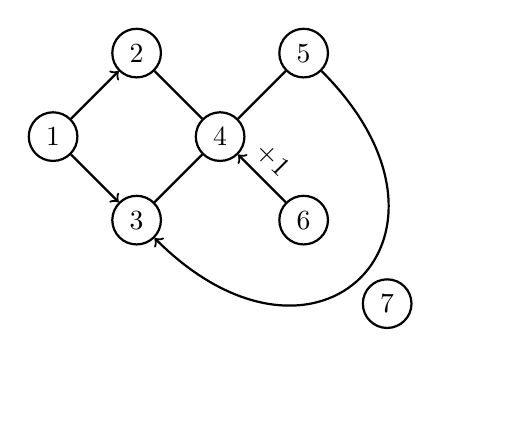
\begin{tikzpicture}[node distance={15mm}, thick, main/.style = {draw, circle}] 
      \node[main] (1) {$1$}; 
      \node[main] (2) [above right of=1] {$2$}; 
      \node[main] (3) [below right of=1] {$3$}; 
      \node[main] (4) [above right of=3] {$4$}; 
      \node[main] (5) [above right of=4] {$5$}; 
      \node[main] (6) [below right of=4] {$6$}; 
      \node[main] (7) [below right of=6] {$7$}; 
      \draw[->] (1) -- (2); 
      \draw[->] (1) -- (3); 
      \draw (2) -- (4); 
      \draw (3) -- (4); 
      \draw (5) -- (4); 
      \draw[->] (5) to [out=315, in=315, looseness=2.5] (3); 
      \draw[->] (6) -- node[midway, above right, sloped, pos=1] {+1} (4); 
      \end{tikzpicture} 
  \end{center}
  

\end{enumerate}

\end{document}